%! Author = rickr
%! Date = 11/17/2021

\section{TSP Better Lower Bound}
    There are problems like the traveling salesman problem in this example
    that are easy to model using branch-and-bound but do not see too much improvements.
    The reason BnB does not work well with TSP is because BnB relies on pseudo
    parallelism, BnB will choose to expand the best possible path each time, and
    with a problem like TSP, the best possible path will almost always be the
    last expanded path. This makes the algorithm almost useless since you
    would expand almost every combination of tour, and essentially brute-force.
    To combat this researchers have used heuristics, in hopes of making a better
    choice for a lower bound.


    \begin{figure}[h]
        \begin{center}
            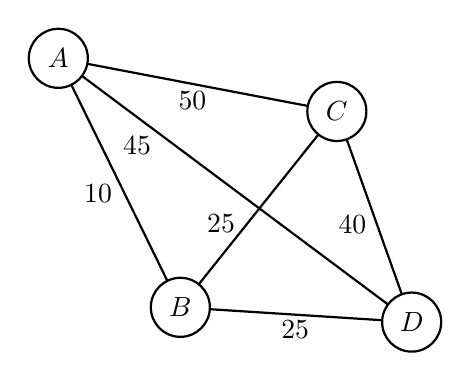
\begin{tikzpicture}[scale=0.125]
                \tikzstyle{every node}+=[inner sep=0pt]
                \draw  [thick](22,-14.2) circle (3);
                \draw  [][thick](22,-14.2) node {$A$};
                \draw  [thick](34.4,-39.5) circle (3);
                \draw  [][thick](34.4,-39.5) node {$B$};
                \draw  [thick](50.3,-19.6) circle (3);
                \draw  [][thick](50.3,-19.6) node {$C$};
                \draw  [thick](57.9,-41) circle (3);
                \draw  [][thick](57.9,-41) node {$D$};
                \draw  [][thick](23.32,-16.89) -- (33.08,-36.81);
                
                \draw [](27.5,-27.94) node [left] {$10$};
                \draw [][thick] (24.95,-14.76) -- (47.35,-19.04);
                
                \draw [](35.62,-17.49) node [below] {$50$};
                \draw [][thick] (51.3,-22.43) -- (56.9,-38.17);
                
                \draw [](53.34,-31.06) node [left] {$40$};
                \draw [][thick] (37.39,-39.69) -- (54.91,-40.81);
                
                \draw [](46.07,-40.81) node [below] {$25$};
                \draw [][thick] (24.4,-15.99) -- (55.5,-39.21);
                
                \draw [](30,-24) node [above] {$45$};
                \draw [][thick] (48.43,-21.94) -- (36.27,-37.16);
                
                \draw [](40, -31) node [left] {$25$};
            \end{tikzpicture}
        \end{center}
        \caption{\doublespacing An example of a TSP Instance}
        \label{fig:lattice}
    \end{figure}

    \subsubsection{Creating a Better Lower Bound}
    Firstly, our lower bound calculation before our heuristic is simply the sum 
    of the tour edges. To improve this we will utilize an encoding scheme known as 
    a graph adjacency matrix, and reduce it. There are two reasons for the reduction, 
    the first is that reduction keeps track of our current state of the tour, and the second
    is that the cost of reduction is an admissible heuristic in the TSP problem.
    The idea is that the cost of reduction is equal to the shortest possible edges left to
    take on the graph. Note, the shortest edges do not have to be constrained to the tour, they
    are just simply the shortest edges coming out of each node. To compute the reduction, take the
    shortest number in each row, then subtract it from each element, finally sum the shortest edges.
    The output matrix becomes the new state of the child branch and used to compute it's lower-bound.\\
    
    \begin{figure}
        \begin{minipage}{.5\linewidth}
          \centering
          \begin{equation*}
            A = 
            \begin{vmatrix}
                \infty & 10 & 50 & 45\\
                10 & \infty & 25 & 25 \\
                50 & 25 & \infty & 40 \\
                45 & 25 & 40 & \infty
	        \end{vmatrix}
          \end{equation*}
          Matrix for TSP instance in Figure 5.
        \end{minipage}%
        \begin{minipage}{.5\linewidth}
          \centering
          \begin{equation*}
	        %!c = 2 + 3 + 2 + 3
            A^{'} = 
                \begin{vmatrix}
                    \infty & 0 & 40 & 35\\
                    0 & \infty & 15 & 15 \\
                    25 & 0 & \infty & 15 \\
                    20 & 0 & 15 & \infty
                \end{vmatrix}
            \end{equation*}
          Row reduced matrix of matrix $A$\\
        \end{minipage}
        \caption{First reduction matrix of TSP instance in Figure 5.
                The cost of reduction $ R(A) = 10 + 10 + 25 + 25 = 70$}
      \end{figure}
      

    After computing the reduction cost we can now make our lower bound calculation.
    \begin{equation}
        LB = LB_p + w(p, n) + R(M_n)
    \end{equation}
    Where $LB_p$ is the lower-bound of the parent, $w(p, n)$ is the weight of the edge
    between the parent, and $R(M_n)$ is the cost of reduction.\\

    \subsubsection{Preformance Gain}
    It is important to realize that branch and bound is not one size fits all algorithm, so
    although there may be a problem that can be encoded with an adjacency matrix, it does not mean
    there exists an admissible heuristic for it. Creating a better lower bound by using a heuristic
    can provide performance gains, but again it is problem dependent.


    \begin{figure}
        \begin{minipage}{.5\linewidth}
          \centering
          \begin{center}
            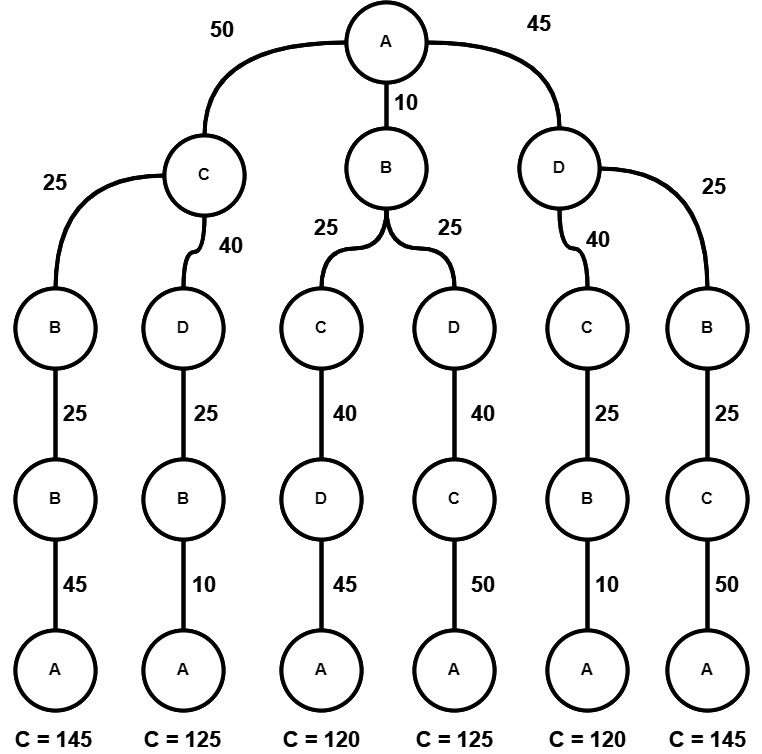
\includegraphics[width=6cm]{images/BnB-TSP-1.jpg}
        \end{center}
        \captionsetup{labelformat=empty}
        \caption{\doublespacing Tree generated without heuristic.}
        \end{minipage}%
        \begin{minipage}{.5\linewidth}
            \centering
            \begin{center}
              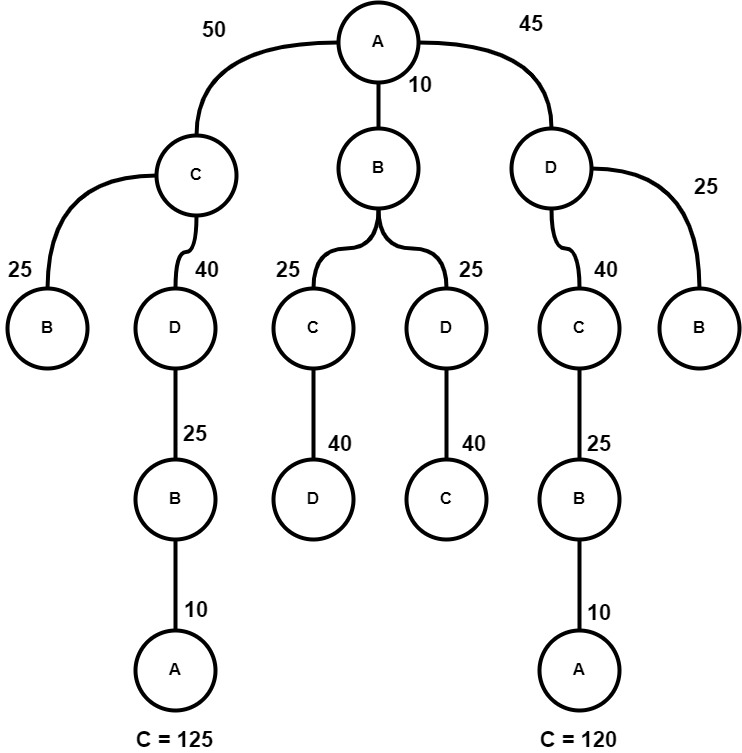
\includegraphics[width=6cm]{images/BnB-TSP-2.jpg}
          \end{center}
          \captionsetup{labelformat=empty}
          \caption{\doublespacing Tree generated with row reduction heuristic.}
          \end{minipage}
        \caption{\doublespacing An example of 
        the trees generated with and without a heuristic for the TSP instance in Figure 5.}
    \end{figure}

   
